\section{Description of Topological Overlap Matrix} \label{ap:tomdefinition}

Starting with a similarity measure $s_{ij}=|cor(i,j)|$ between node $i$ and node $j$, one could apply a hard threshold to determine if this pair is considered connected or not resulting in an un-weighted network (a matrix of 0's and 1's). Instead, Zhang and Horvath~\citep{zhang2005general} propose a soft thresholding framework that assigns a connection weight to each gene pair using a power adjacency function $a_{ij} = |s_{ij}|^{\beta}$. The parameter $\beta$ determines the sensitivity and specificity of the pairwise connection strengths e.g. a larger $\beta$ will result in fewer connected nodes which can reduce noise in the network but can also eliminate signal if too large. A measure of similarity is then derived using the symmetric and non-negative topological overlap matrix~\citep{ravasz2002hierarchical} (TOM) $\Omega = [\omega_{ij}]$:
\begin{equation}
\omega_{ij} = \frac{l_{ij} + a_{ij}}{min\left\lbrace k_i, k_j \right\rbrace + 1-a_{ij} }  \label{eq:TOM}
\end{equation}
where $l_{ij} = \sum_u a_{iu}a_{uj}$, $k_i = \sum_u a_{iu}$ is the node connectivity, and the index $u$ runs across all nodes of the network. Basically, $\omega_{ij}$ is a measure of similarity in terms of the commonality of the nodes they connect to. If $i$ and $j$ are unconnected and do not share any neighbors then $\omega_{ij}=0$. An $\omega_{ij}=1$ means that $i$ and $j$ are connected, and the neighbors of the node with fewer connections are also neighbors of the other node. 


\section{Binary Outcome Simulation Results}\label{ap:binaryoutcome}

\begin{figure}[H]
	\centering
	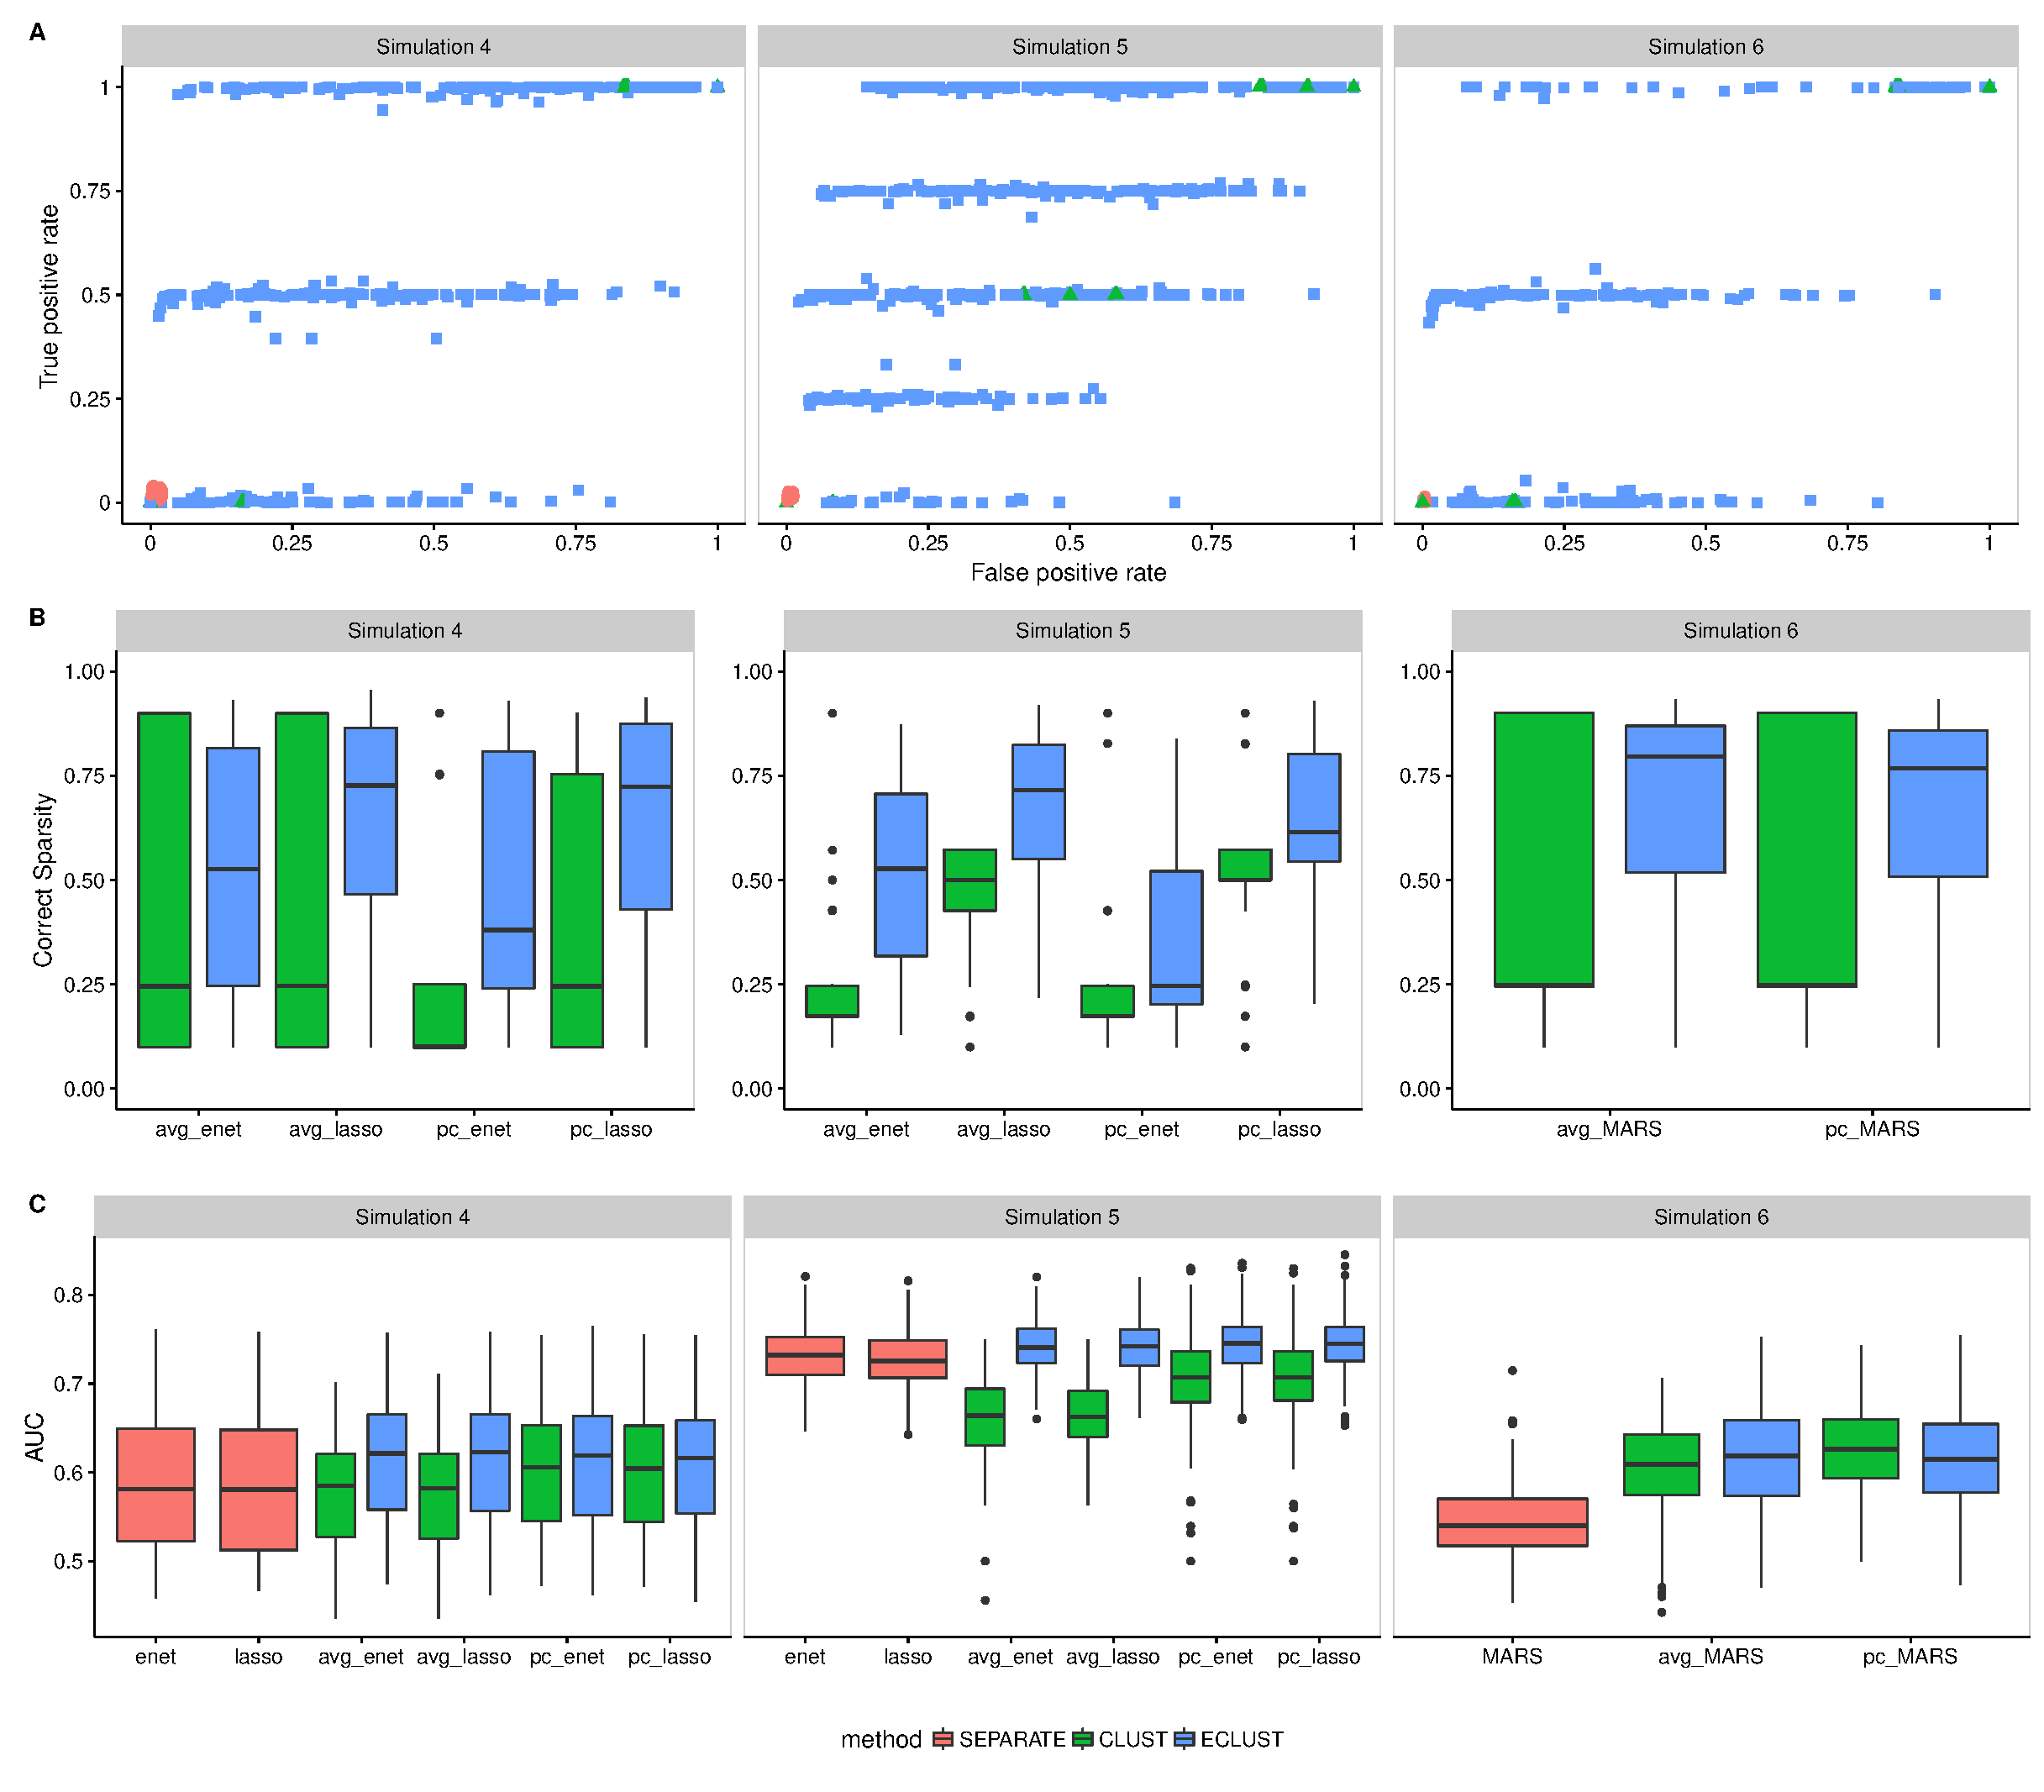
\includegraphics[scale=0.40, keepaspectratio]{./figs/guillimin/results/figures/sim4-5-6-combined/modelfit_sim456.eps}
	%\caption{Model fit results from simulations 4, 5 and 6 for $SNR=1$, $\rho = 0.9$, and \mbox{$\alpha_{j} \sim \tm{Unif}\left[\log(1.9), \log(2.1)\right]$}. SEPARATE results are in pink, CLUST in green and ECLUST in blue.}
	\caption{Model fit results from simulations 4, 5 and 6 for $SNR=1$, $\rho = 0.9$, and \mbox{$\alpha_{j} \sim \tm{Unif}\left[\log(1.9), \log(2.1)\right]$}. SEPARATE results are in pink, CLUST in green and ECLUST in blue.}
	\label{fig:sim-modelfit456}
\end{figure}

\begin{figure}[H]
	\centering
	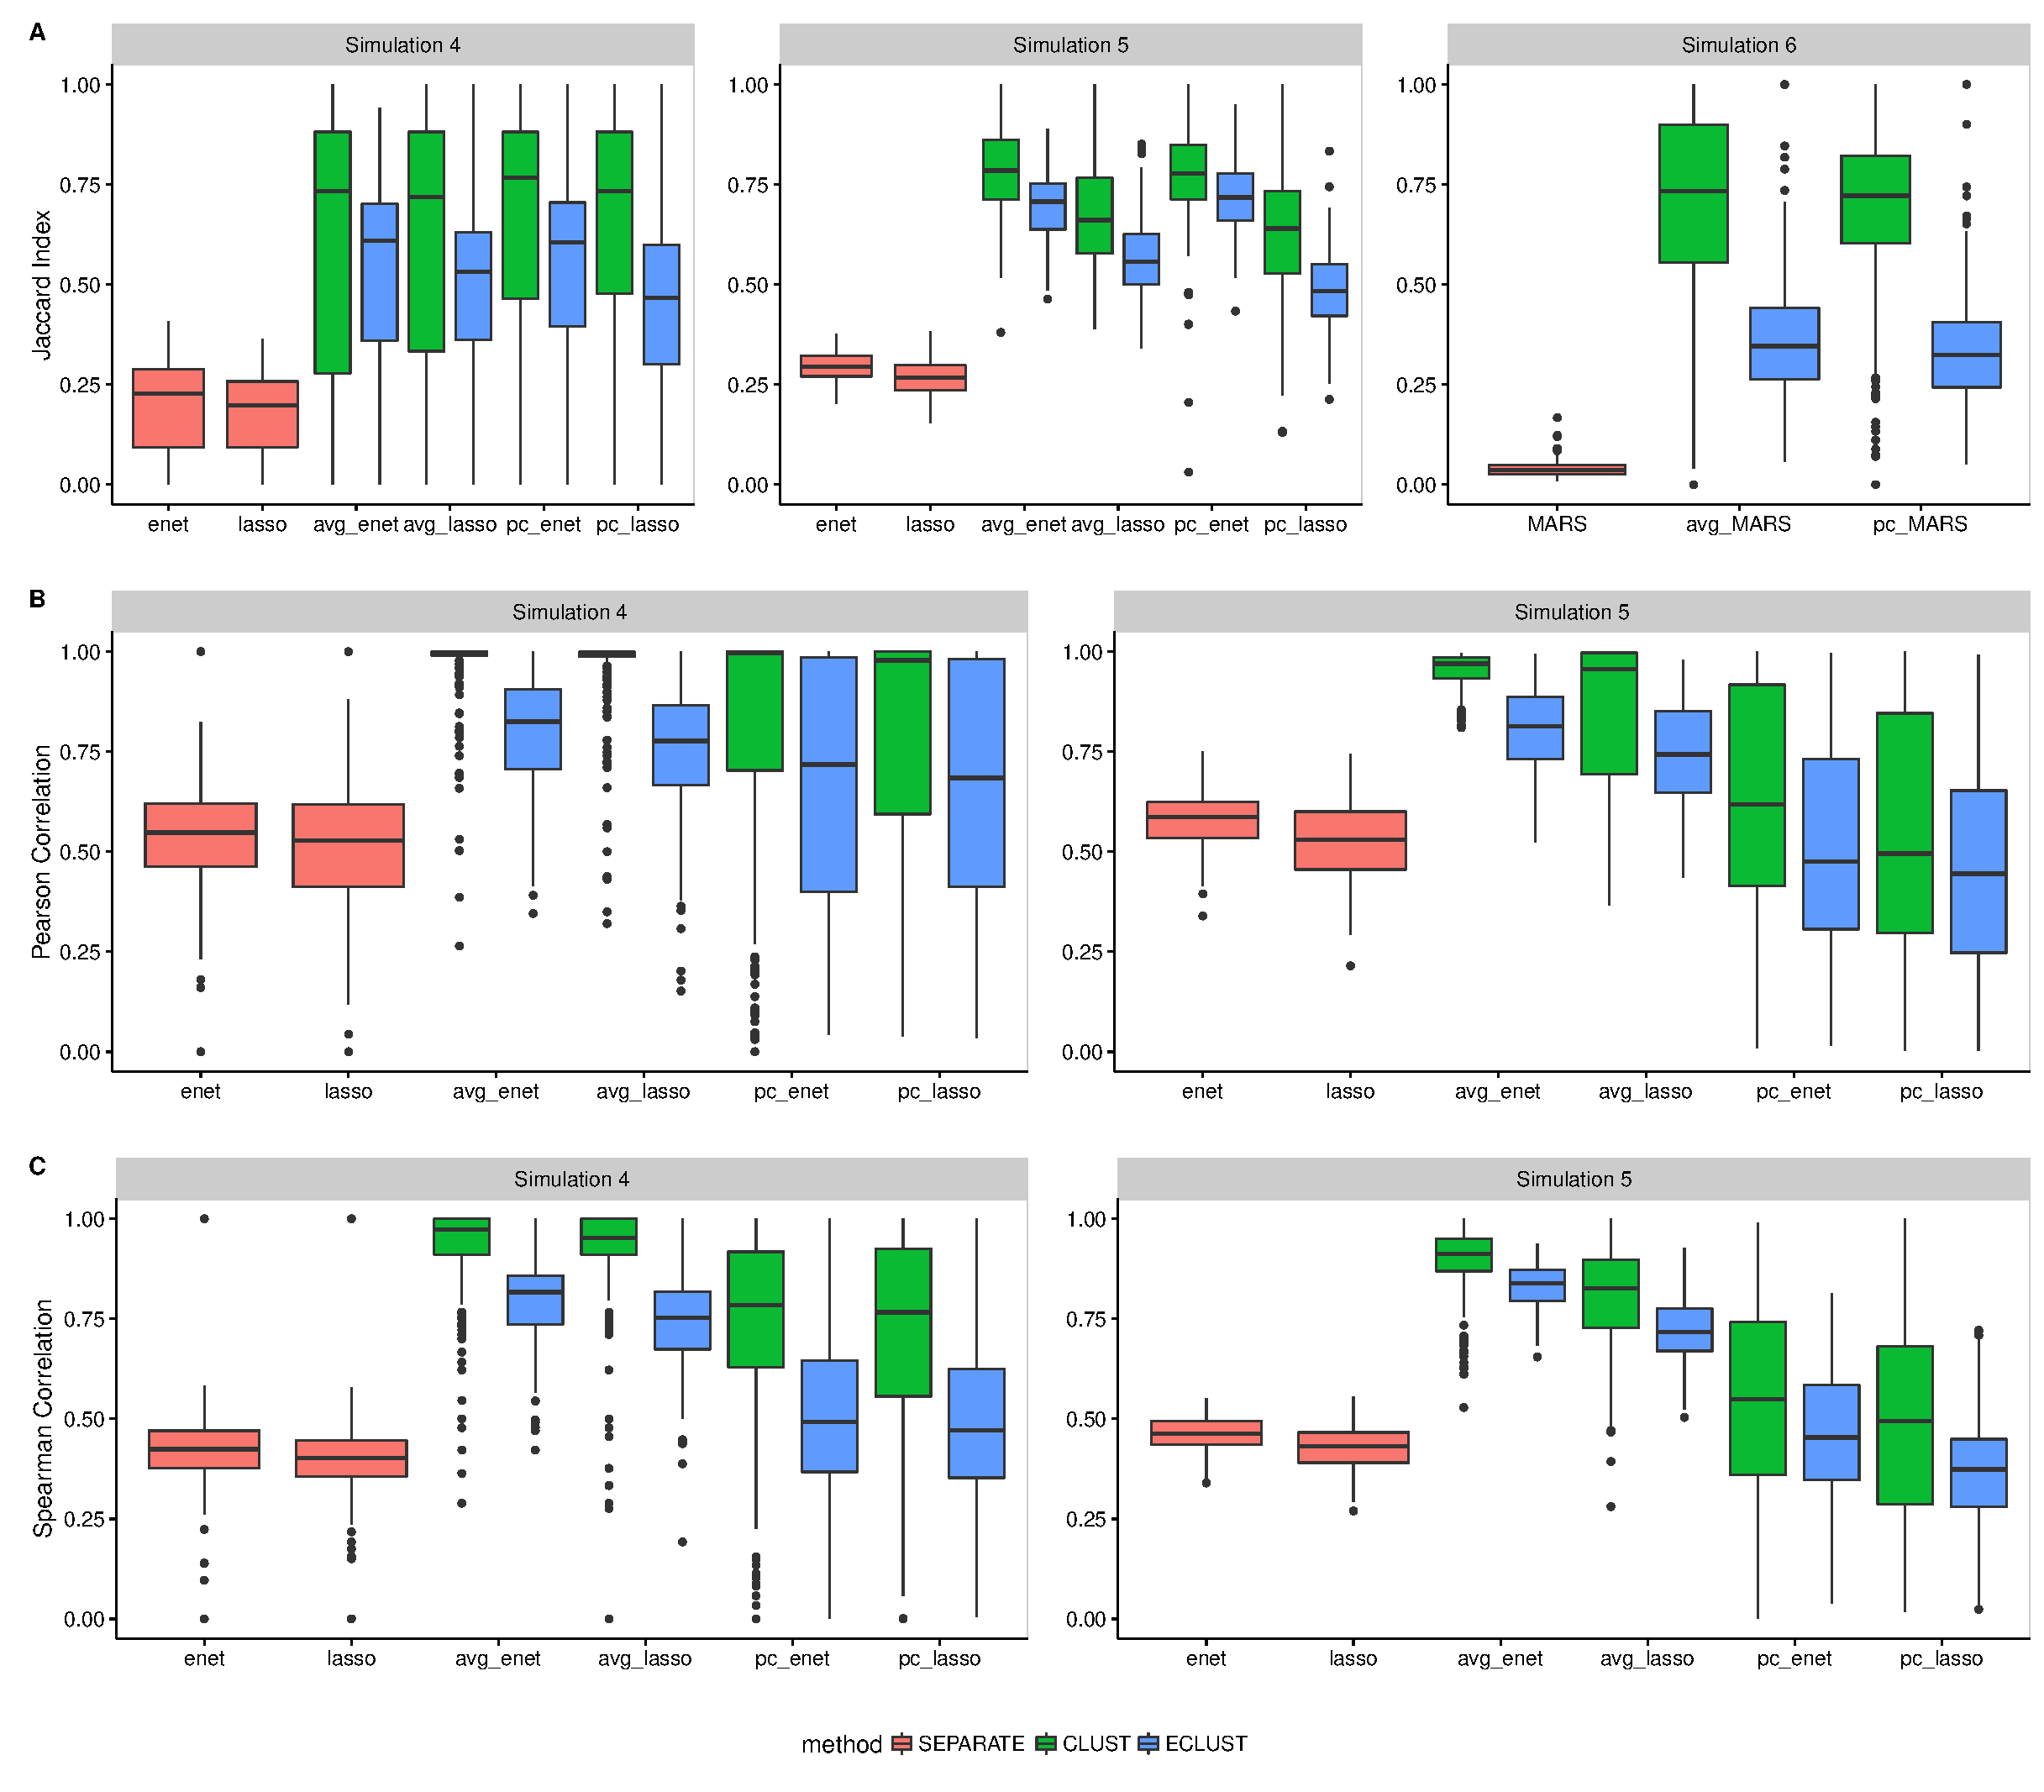
\includegraphics[scale=0.40, keepaspectratio]{./figs/guillimin/results/figures/sim4-5-6-combined/stability_sim456.eps}
	\caption{Stability results from simulations 4, 5 and 6 for $SNR=1$, $\rho = 0.9$, and \mbox{$\alpha_{j} \sim \tm{Unif}\left[\log(1.9), \log(2.1)\right]$}. SEPARATE results are in pink, CLUST in green and ECLUST in blue.}
	\label{fig:sim-stability456}
\end{figure}

\begin{figure}[H]
	\centering
	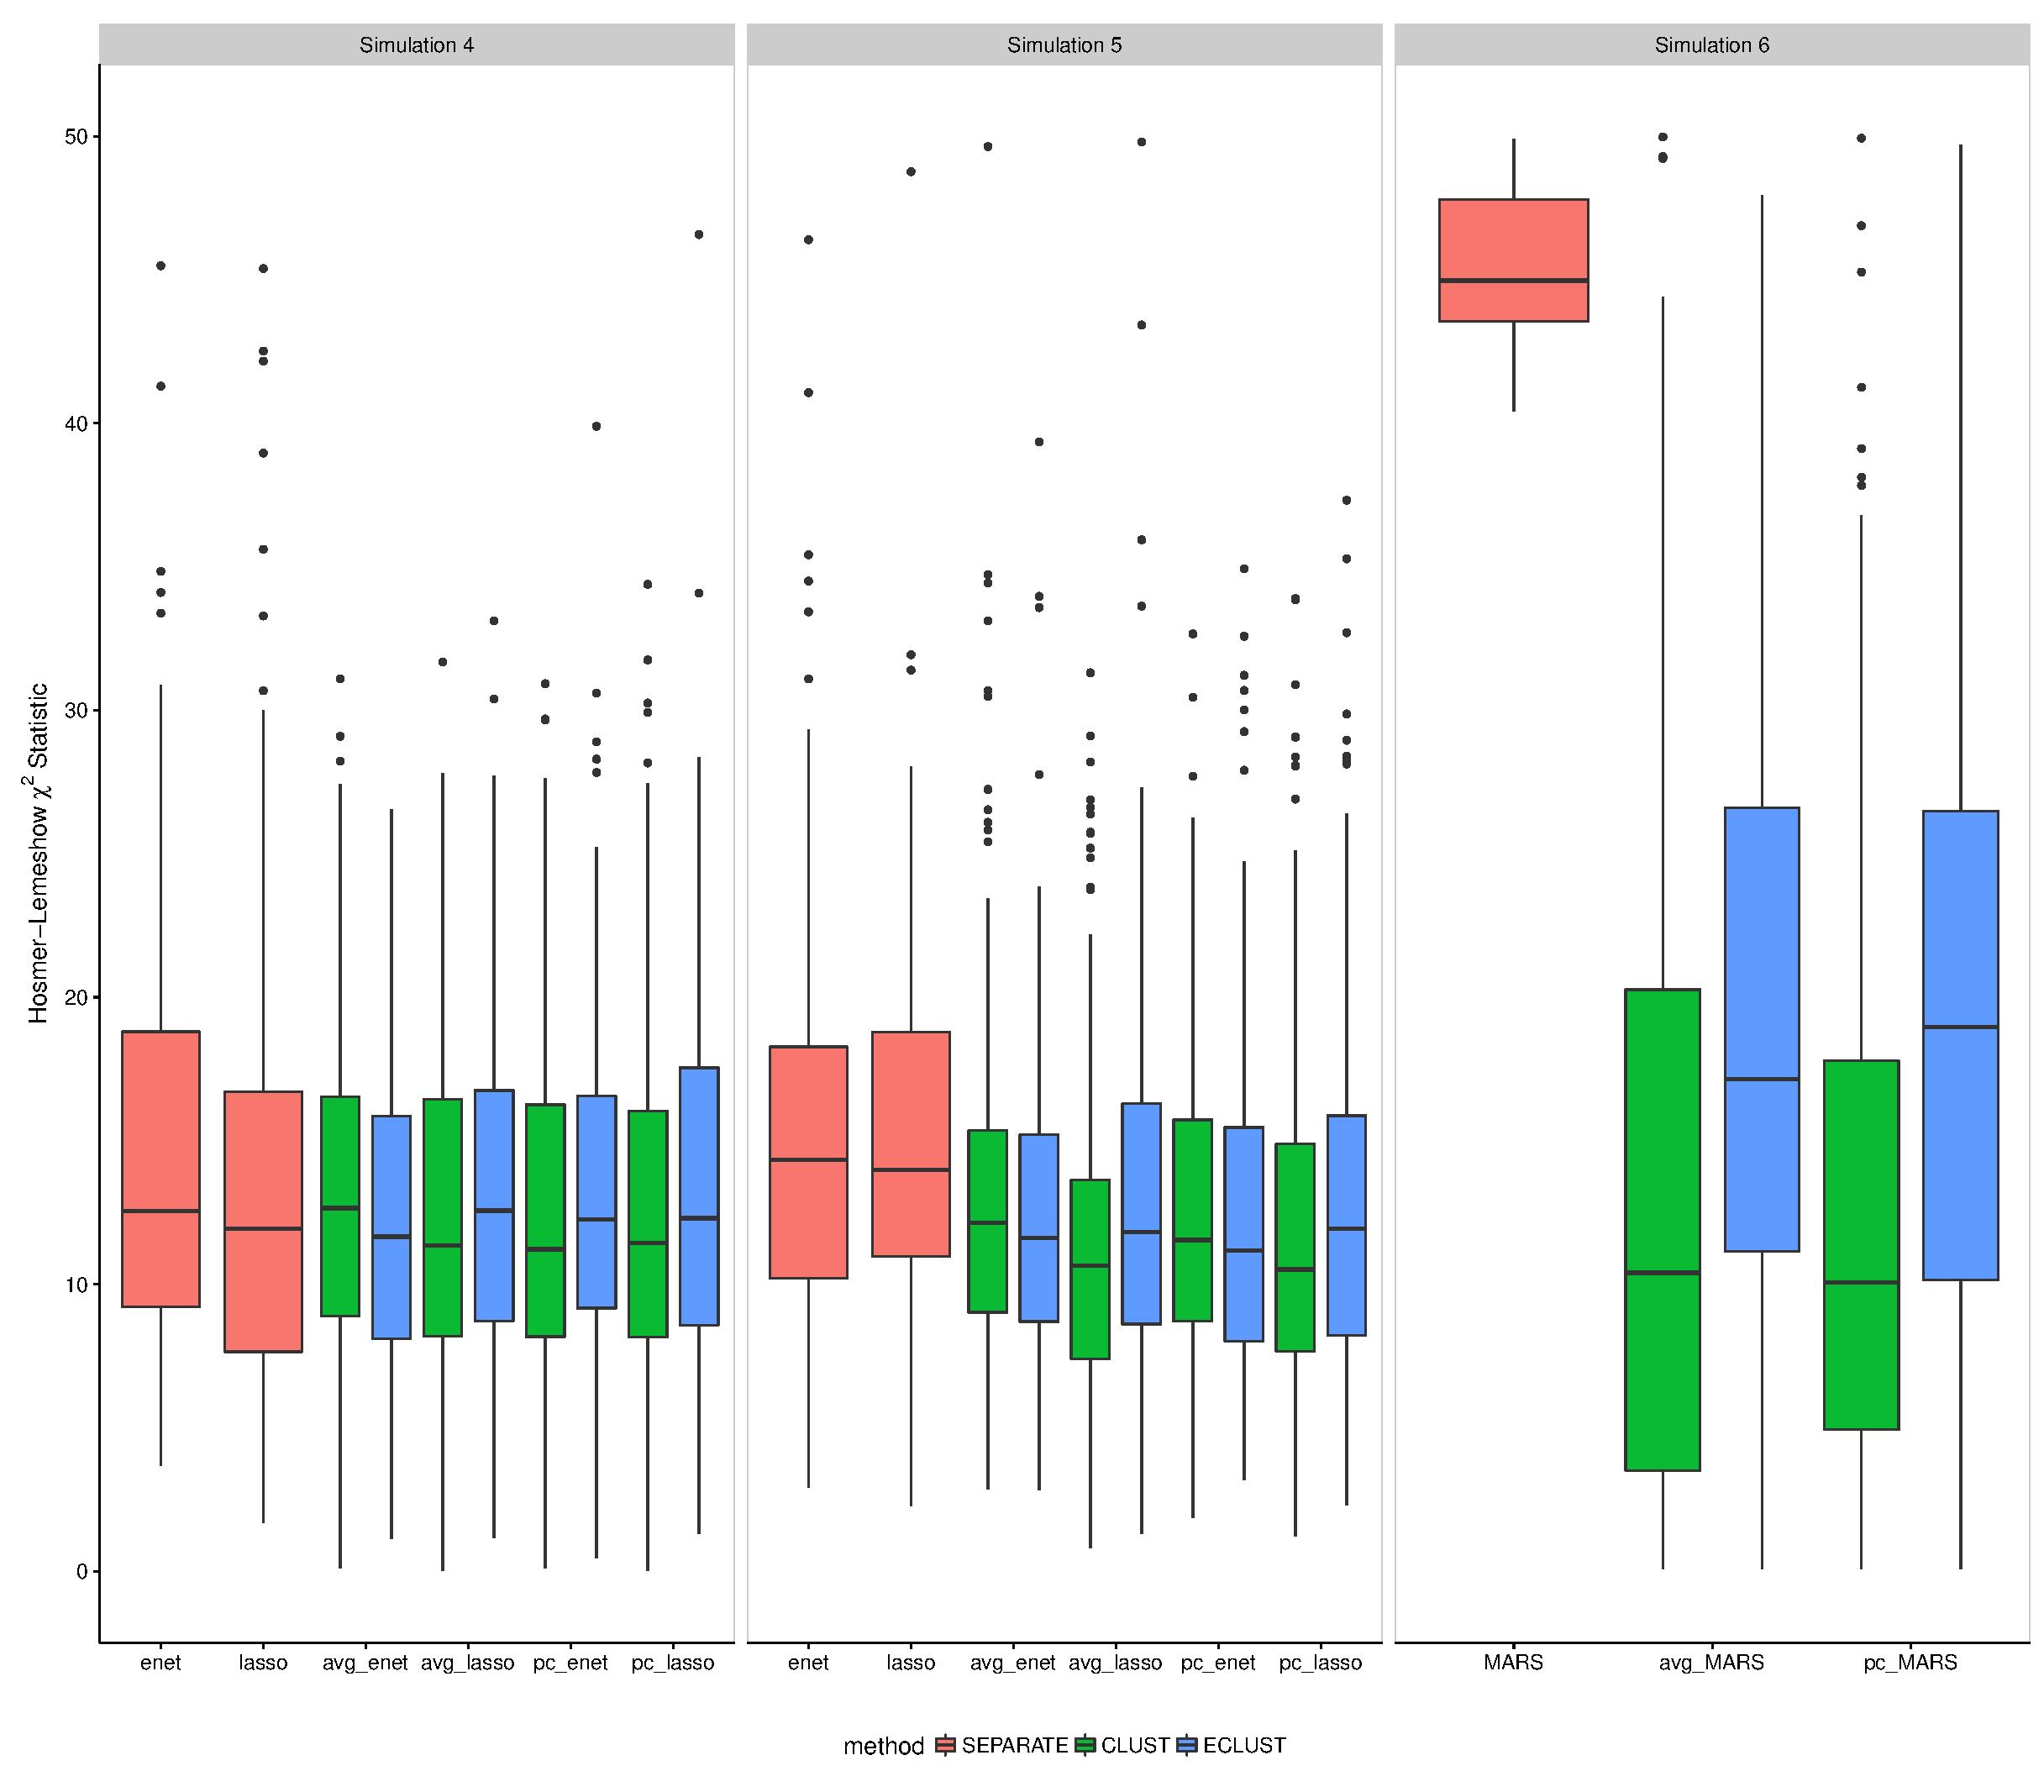
\includegraphics[scale=0.40, keepaspectratio]{./figs/guillimin/results/figures/sim4-5-6-combined/calibration_sim456.eps}
	\caption{Hosmer-Lemeshow statistics from simulations 4, 5 and 6 for $SNR=1$, $\rho = 0.9$, and \mbox{$\alpha_{j} \sim \tm{Unif}\left[\log(1.9), \log(2.1)\right]$}. SEPARATE results are in pink, CLUST in green and ECLUST in blue.}
	\label{fig:sim-calibration456}
\end{figure}


\begin{figure}[H]
	\centering
	\includegraphics[width=1\linewidth]{./figs/guillimin/results/figures/sim4-5-6-combined/calibration-pvalue_sim4.eps}
	\caption{Hosmer-Lemeshow p-values from simulation 4 for $SNR=1$, $\rho = 0.9$, and \mbox{$\alpha_{j} \sim \tm{Unif}\left[\log(1.9), \log(2.1)\right]$}. SEPARATE results are in pink, CLUST in green and ECLUST in blue.}
	\label{fig:sim-calibrationhist4}
\end{figure}


\begin{figure}[H]
	\centering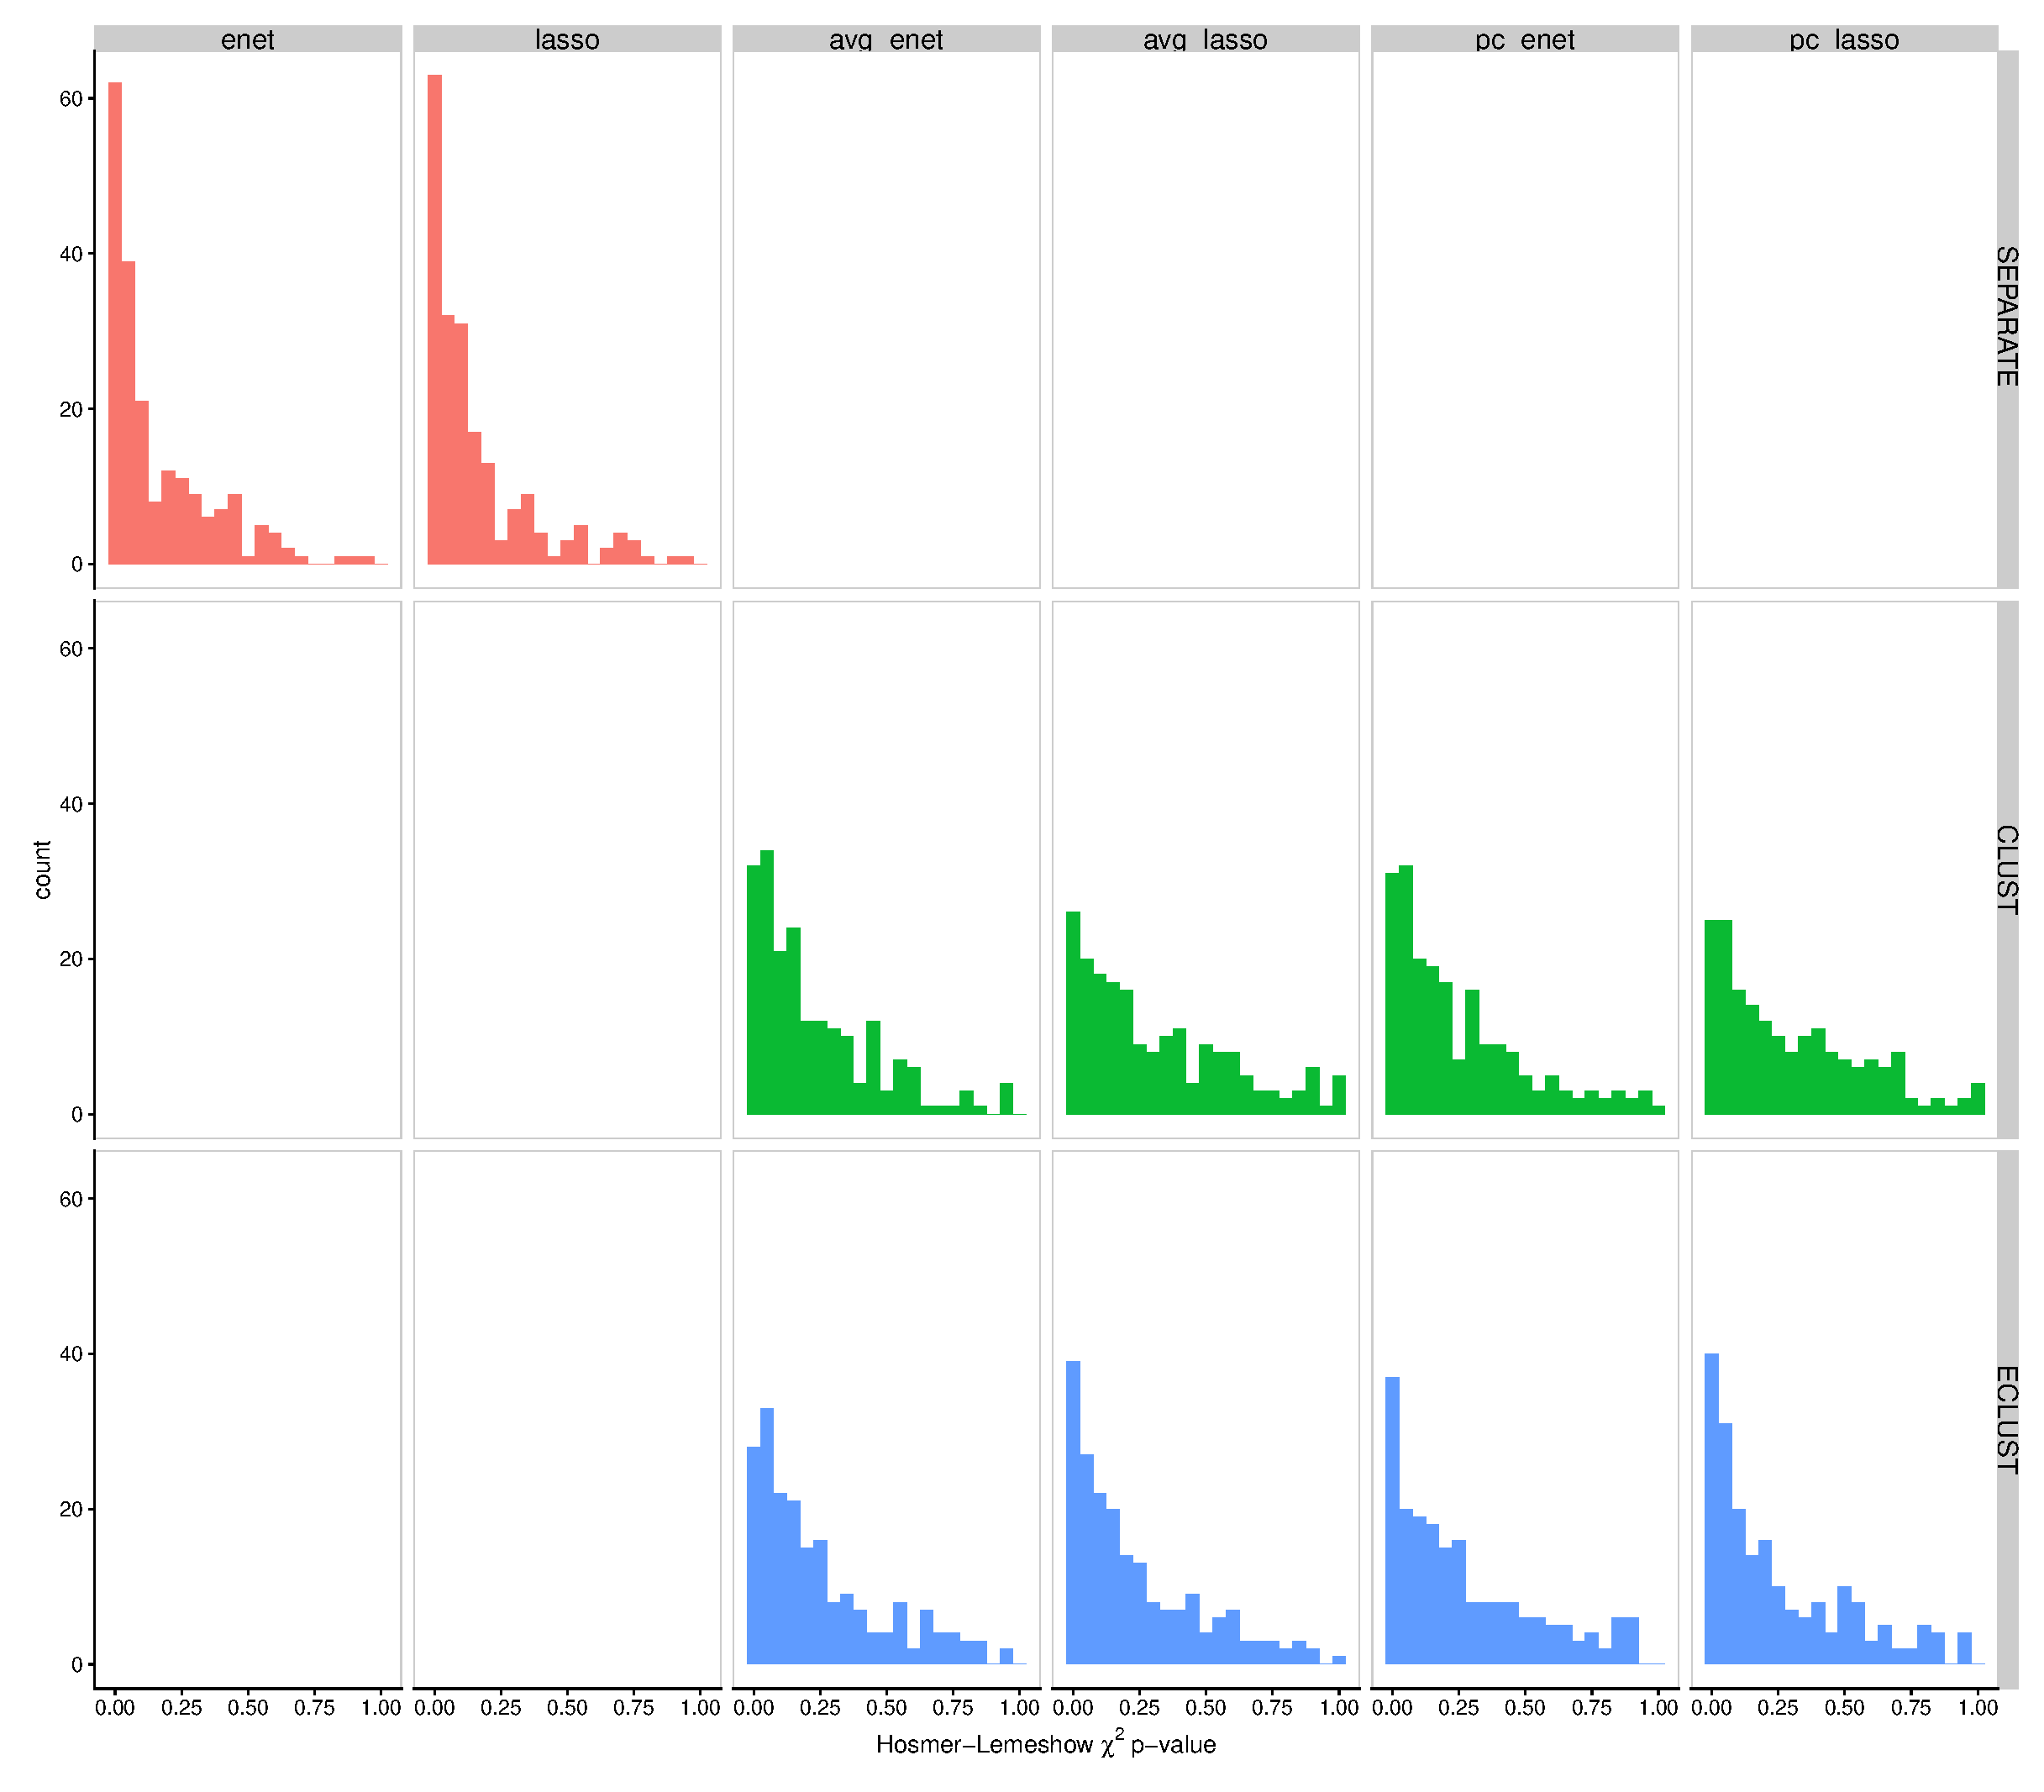
\includegraphics[width=1\linewidth]{./figs/guillimin/results/figures/sim4-5-6-combined/calibration-pvalue_sim5.eps}
	\caption{Hosmer-Lemeshow p-values from simulation 5 for $SNR=1$, $\rho = 0.9$, and \mbox{$\alpha_{j} \sim \tm{Unif}\left[\log(1.9), \log(2.1)\right]$}. SEPARATE results are in pink, CLUST in green and ECLUST in blue.}\label{fig:sim-calibrationhist5}
\end{figure}

\begin{figure}[H]
	\centering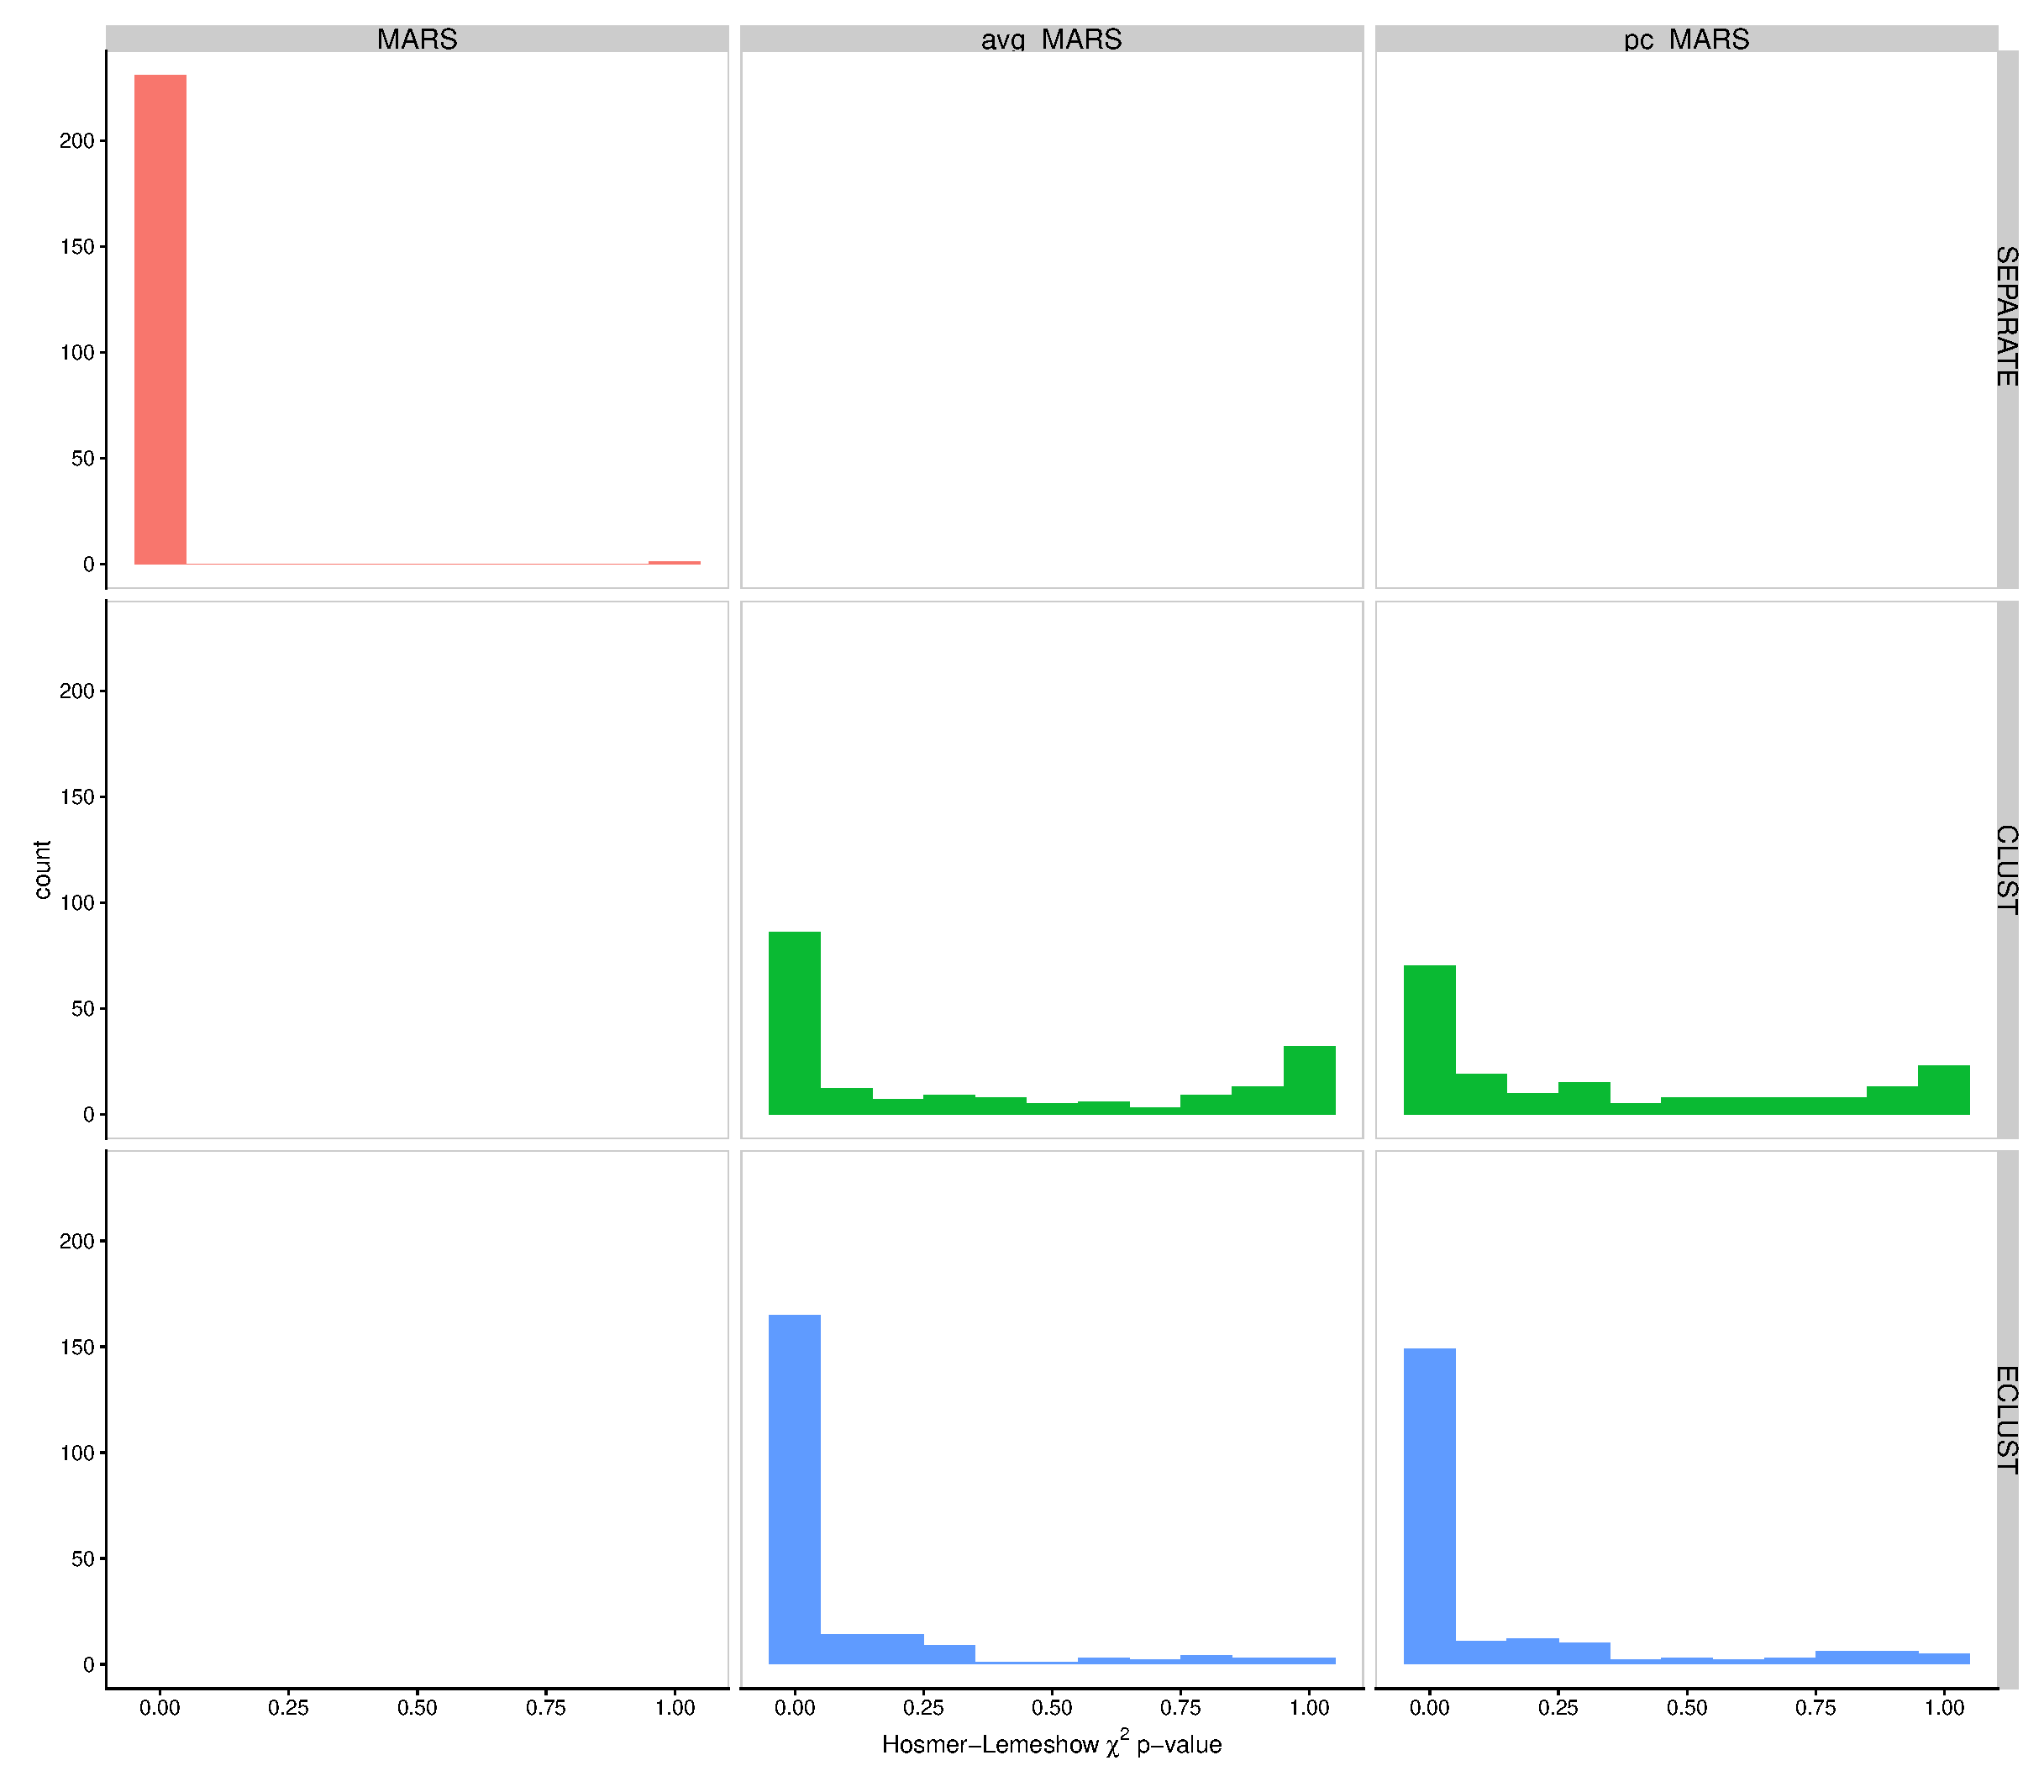
\includegraphics[width=1\linewidth]{./figs/guillimin/results/figures/sim4-5-6-combined/calibration-pvalue_sim6.eps}
	\caption{Hosmer-Lemeshow p-values from simulation 6 for $SNR=1$, $\rho = 0.9$, and \mbox{$\alpha_{j} \sim \tm{Unif}\left[\log(1.9), \log(2.1)\right]$}. SEPARATE results are in pink, CLUST in green and ECLUST in blue.}\label{fig:sim-calibrationhist6}
\end{figure}


\section{Analysis of Clusters}\label{ap:clusters}

\begin{figure}[H]
	\centering
	\includegraphics[scale=0.9, keepaspectratio]{./figs/figures-for-manuscript/nclusters.png}
	\caption{Number of estimated clusters from applying the \texttt{dynamicTreeCut} algorithm to hierarchical clustering of the dissimilarity matrix with average linkage. \mbox{Left panel}: CLUST uses $1-Cor(X_{all})$ and ECLUST uses the euclidean distance of $Cor(X_{\tm{diff}})$ as measures of dissimilarity. Right panel: CLUST uses $1-TOM(X_{all})$ and ECLUST uses the euclidean distance of $TOM(X_{\tm{diff}})$ as measures of dissimilarity. Empirical distributions based on 200 simulation runs.}
	\label{fig:compare_clusters}
\end{figure}


\begin{figure}[H]
	\centering
	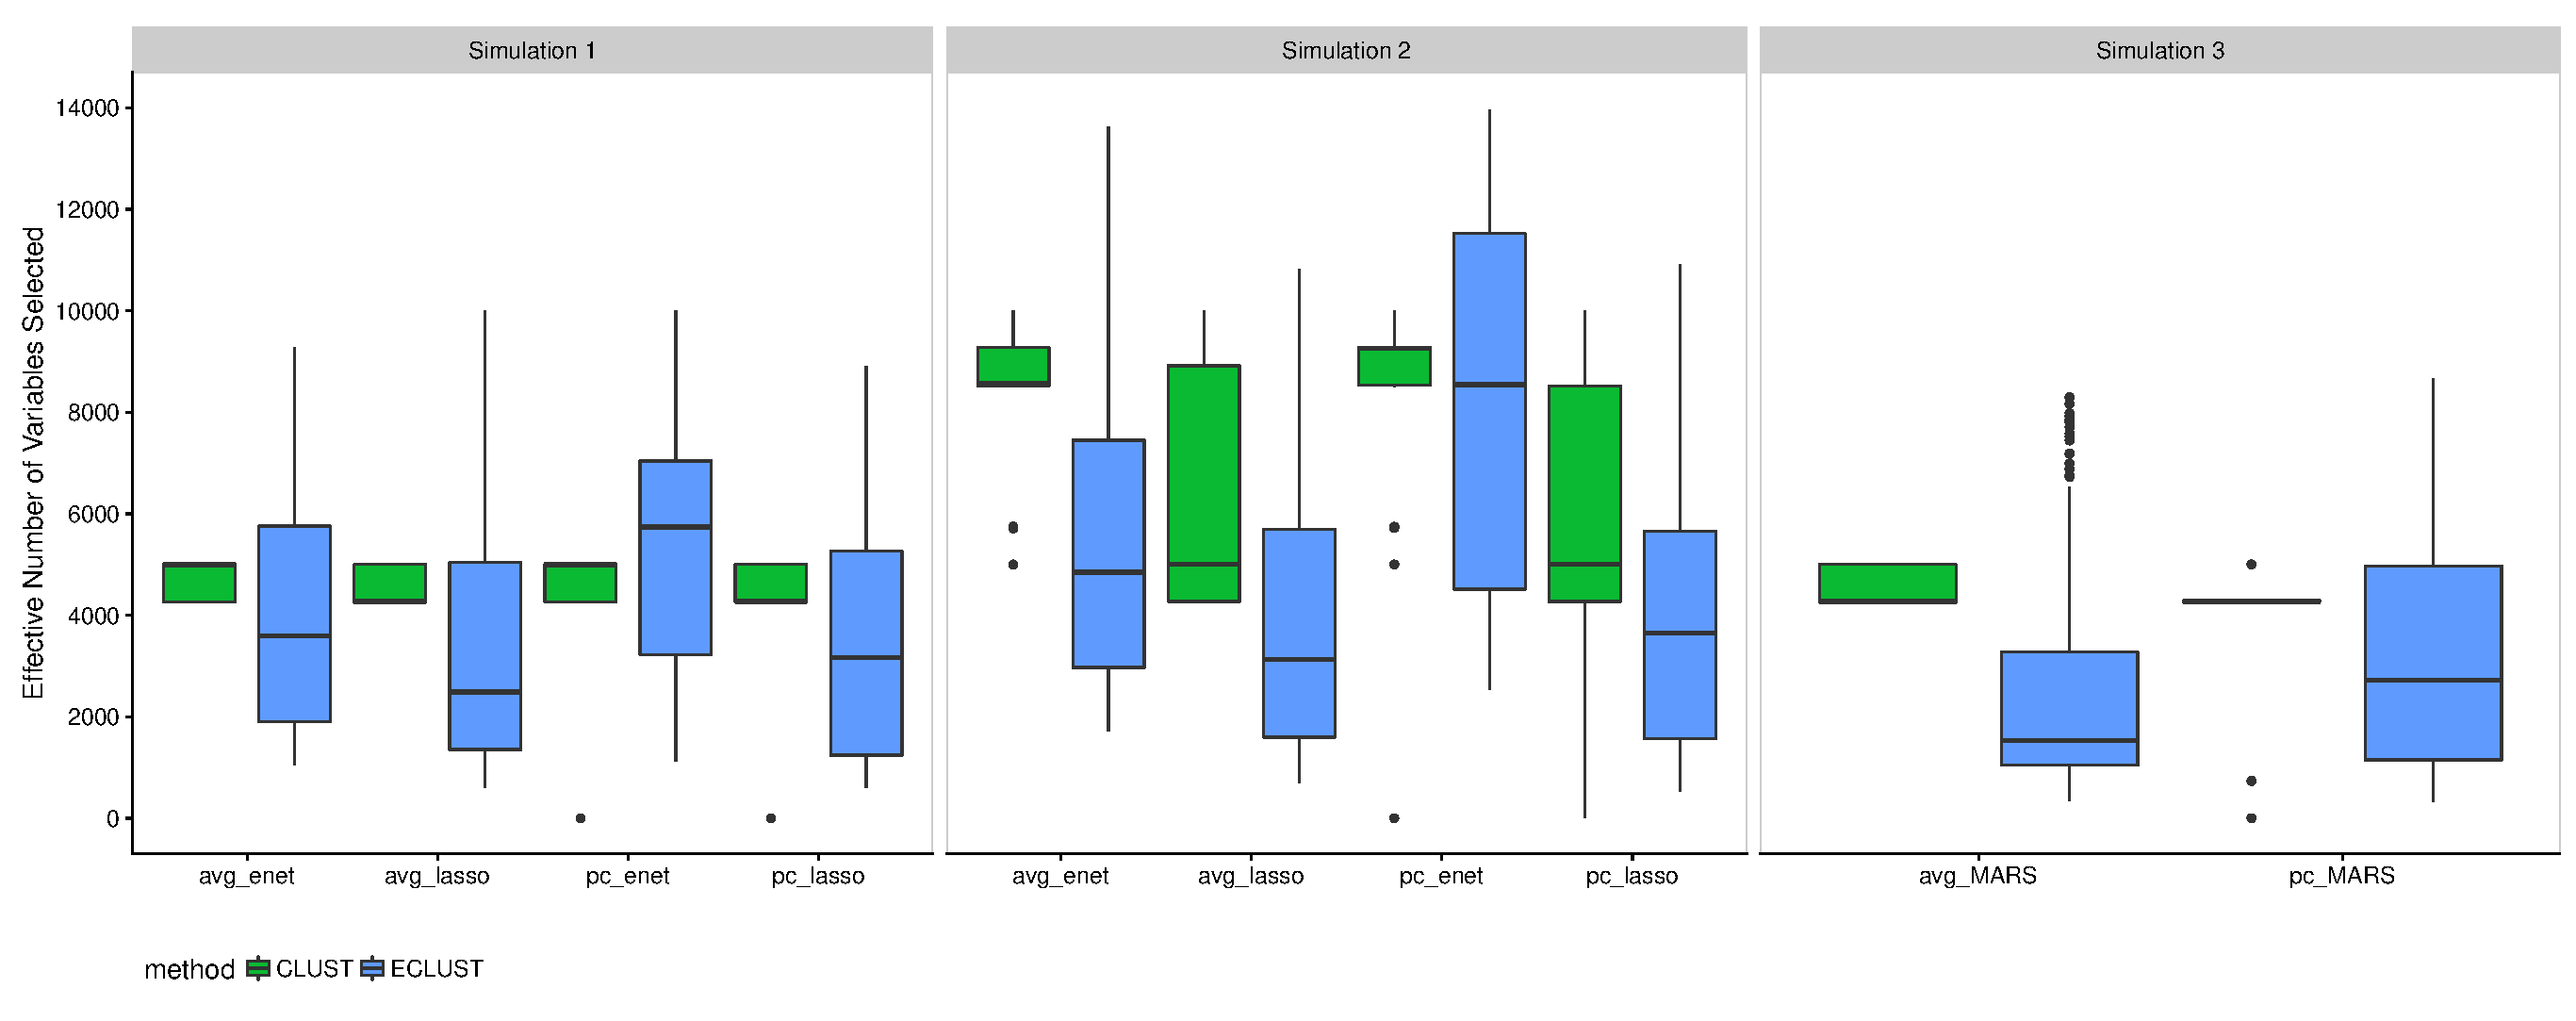
\includegraphics[width=1\linewidth, keepaspectratio]{./figs/guillimin/results/figures/sim4-5-6-combined/Shat_sim123.eps}
	\caption{Effective number of selected variables for simulations 1-3 for $SNR = 1, \rho=0.9$. A variable was considered ``selected'' if its corresponding cluster representative was selected.}
	\label{fig:compare_clusters2}
\end{figure}

\begin{figure}[H]
	\centering
	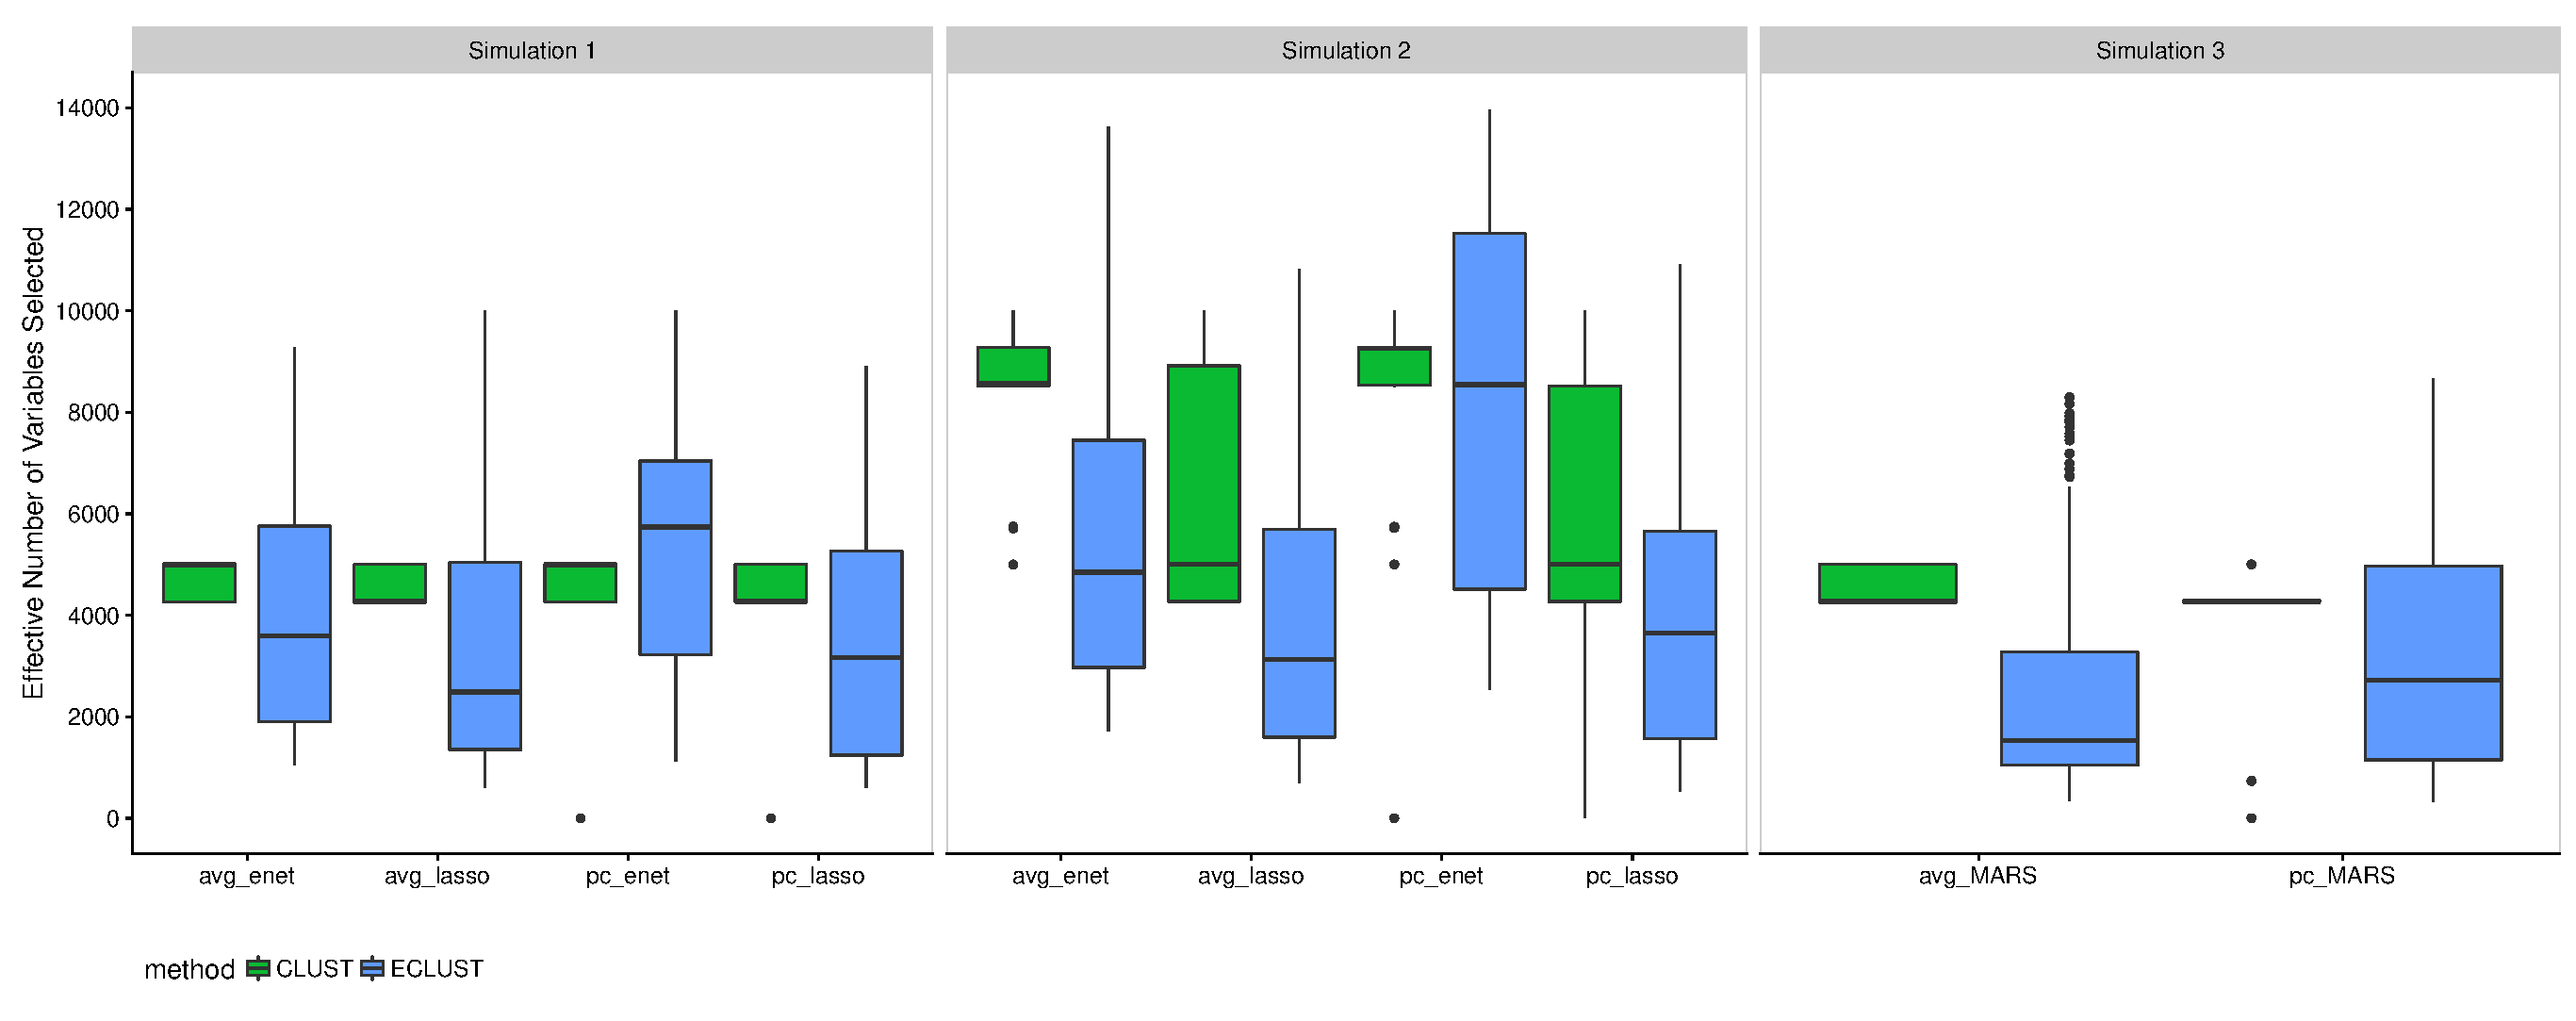
\includegraphics[width=1\linewidth, keepaspectratio]{./figs/guillimin/results/figures/sim4-5-6-combined/Shat_sim123.eps}
	\caption{Effective number of selected variables for simulations 4-6 for $SNR = 1, \rho=0.9$ and \mbox{$\alpha_{j} \sim \tm{Unif}\left[\log(1.9), \log(2.1)\right]$}. A variable was considered ``selected'' if its corresponding cluster representative was selected.}
	\label{fig:compare_clusters3}
\end{figure}


\section{Simulation Results Using TOM as a Measure of Similarity} \label{ap:sim-TOM}


\subsection*{Simulation 1}

\begin{figure}[H]
	\centering
	\includegraphics[scale=0.6, keepaspectratio]{./figs/hydra/results/figures/sim1-sept10/RMSE_TOM_sim1.png}
	\caption{Simulation 1 -- Root mean squared error on an independent test set using the TOM as a measure of similarity from 200 simulation runs. Vertical panels represent varying correlation between active clusters. Horizontal panels represent different signal-to-noise ratios.}
	\label{fig:RMSE_TOM_sim1}
\end{figure}

\begin{figure}[H]
	\centering
	\includegraphics[scale=0.6, keepaspectratio]{./figs/hydra/results/figures/sim1-sept10/CorrectSparsity_TOM_sim1.png}
	\caption{Simulation 1 -- Correct Sparsity based on the training set using the TOM as a measure of similarity from 200 simulation runs. Vertical panels represent varying correlation between active clusters. Horizontal panels represent different signal-to-noise ratios.}
	\label{fig:CorrectSparsity_TOM_sim1}
\end{figure}


\begin{figure}
	\includegraphics[scale=0.6, keepaspectratio]{./figs/hydra/results/figures/sim1-sept10/tpr_fpr_TOM_sim1.png}
	\caption{Simulation 1 -- True positive rate vs. false positive rate based on the training set using the TOM as a measure of similarity. Each point represents 1 simulation run (there are a total of 200 simulation runs). Vertical panels represent varying correlation between active clusters. Horizontal panels represent different signal-to-noise ratios.}
	\label{fig:tpr_fpr_TOM_sim1}
\end{figure}


\begin{figure}[H]
	\centering
	\includegraphics[scale=0.6, keepaspectratio]{./figs/hydra/results/figures/sim1-sept10/jacc_TOM_sim1.png}
	\caption{Simulation 1 -- Average Jaccard Index from 10 CV folds of the training set using the TOM as a measure of similarity. We fit the model to each of the 10 CV folds resulting in 10 sets of selected predictors. We then calculate the Jaccard Index between all $\binom{10}{2}$ possible combinations of these sets and take the average. This process is repeated for each of the 200 simulation runs. Vertical panels represent varying correlation between active clusters. Horizontal panels represent different signal-to-noise ratios.}
	\label{fig:jacc_TOM_sim1}
\end{figure}


\begin{figure}[H]
	\centering
	\includegraphics[scale=0.6, keepaspectratio]{./figs/hydra/results/figures/sim1-sept10/spearman_TOM_sim1.png}
	\caption{Simulation 1 -- Average Spearman correlation from 10 CV folds of the training set using the TOM as a measure of similarity. We fit the model to each of the 10 CV folds resulting in 10 sets of estimated regression coefficients. We then calculate the Spearman correlation between all $\binom{10}{2}$ possible combinations of these sets and take the average. This process is repeated for each of the 200 simulation runs. Vertical panels represent varying correlation between active clusters. Horizontal panels represent different signal-to-noise ratios.}
	\label{fig:spearman_TOM_sim1}
\end{figure}


\begin{figure}[H]
	\centering
	\includegraphics[scale=0.6, keepaspectratio]{./figs/hydra/results/figures/sim1-sept10/pearson_TOM_sim1.png}
	\caption{Simulation 1 -- Average Pearson correlation from 10 CV folds of the training set using the TOM as a measure of similarity. We fit the model to each of the 10 CV folds resulting in 10 sets of estimated regression coefficients. We then calculate the Pearson correlation between all $\binom{10}{2}$ possible combinations of these sets and take the average. This process is repeated for each of the 200 simulation runs. Vertical panels represent varying correlation between active clusters. Horizontal panels represent different signal-to-noise ratios.}
	\label{fig:pearson_TOM_sim1}
\end{figure}

\subsection*{Simulation 2}
\begin{figure}[H]
	\centering
	\includegraphics[scale=0.55, keepaspectratio]{./figs/hydra/results/figures/sim2-sept8/RMSE_TOM_sim2.png}
	\caption{Simulation 2 -- Root mean squared error on an independent test set using the TOM as a measure of similarity from 200 simulation runs. \mbox{(A) $\alpha_{j} \sim \tm{Unif}\left[0.4, 0.6\right]$}, \mbox{(B) $\alpha_{j} \sim \tm{Unif}\left[1.9, 2.1\right]$}. Vertical panels represent varying correlation between active clusters. Horizontal panels represent different signal-to-noise ratios.}
	\label{fig:RMSE_TOM_sim2}
\end{figure}

\begin{figure}[H]
	\centering
	\includegraphics[scale=0.58, keepaspectratio]{./figs/hydra/results/figures/sim2-sept8/CorrectSparsity_TOM_sim2.png}
	\caption{Simulation 2 -- Correct Sparsity based on the training set using the TOM as a measure of similarity from 200 simulation runs. \mbox{(A) $\alpha_{j} \sim \tm{Unif}\left[0.4, 0.6\right]$}, \mbox{(B) $\alpha_{j} \sim \tm{Unif}\left[1.9, 2.1\right]$}. Vertical panels represent varying correlation between active clusters. Horizontal panels represent different signal-to-noise ratios.}
	\label{fig:CorrectSparsity_TOM_sim2}
\end{figure}


\begin{figure}
	\includegraphics[scale=0.57, keepaspectratio]{./figs/hydra/results/figures/sim2-sept8/tpr_fpr_TOM_sim2.png}
	\caption{Simulation 2 -- True positive rate vs. false positive rate based on the training set using the TOM as a measure of similarity. \mbox{(A) $\alpha_{j} \sim \tm{Unif}\left[0.4, 0.6\right]$}, \mbox{(B) $\alpha_{j} \sim \tm{Unif}\left[1.9, 2.1\right]$}. Each point represents 1 simulation run (there are a total of 200 simulation runs). Vertical panels represent varying correlation between active clusters. Horizontal panels represent different signal-to-noise ratios.}
	\label{fig:tpr_fpr_TOM_sim2}
\end{figure}

%\begin{sidewaysfigure}
%	\includegraphics[width=0.9\columnwidth]{./hydra/results/figures/sim2-sept8/tpr_fpr_alpha2sim2.png}
%	\caption{True positive rate vs. false positive rate for $\alpha_{jE} \sim \tm{Unif}\left[1.9, 2.1\right]$}
%	\label{fig:sim2-corvstom2}
%\end{sidewaysfigure}


\begin{figure}[H]
	\centering
	\includegraphics[scale=0.55, keepaspectratio]{./figs/hydra/results/figures/sim2-sept8/jacc_TOM_sim2.png}
	\caption{Simulation 2 -- Average Jaccard Index from 10 CV folds of the training set using the TOM as a measure of similarity. \mbox{(A) $\alpha_{j} \sim \tm{Unif}\left[0.4, 0.6\right]$}, \mbox{(B) $\alpha_{j} \sim \tm{Unif}\left[1.9, 2.1\right]$}. We fit the model to each of the 10 CV folds resulting in 10 sets of selected predictors. We then calculate the Jaccard Index between all $\binom{10}{2}$ possible combinations of these sets and take the average. This process is repeated for each of the 200 simulation runs. Vertical panels represent varying correlation between active clusters. Horizontal panels represent different signal-to-noise ratios.}
	\label{fig:jacc_TOM_sim2}
\end{figure}


\begin{figure}[H]
	\centering
	\includegraphics[scale=0.52, keepaspectratio]{./figs/hydra/results/figures/sim2-sept8/spearman_TOM_sim2.png}
	\caption{Simulation 2 -- Average Spearman correlation from 10 CV folds of the training set using the TOM as a measure of similarity. \mbox{(A) $\alpha_{j} \sim \tm{Unif}\left[0.4, 0.6\right]$}, \mbox{(B) $\alpha_{j} \sim \tm{Unif}\left[1.9, 2.1\right]$}. We fit the model to each of the 10 CV folds resulting in 10 sets of estimated regression coefficients. We then calculate the Spearman correlation between all $\binom{10}{2}$ possible combinations of these sets and take the average. This process is repeated for each of the 200 simulation runs. Vertical panels represent varying correlation between active clusters. Horizontal panels represent different signal-to-noise ratios.}
	\label{fig:spearman_TOM_sim2}
\end{figure}

\begin{figure}[H]
	\centering
	\includegraphics[scale=0.55, keepaspectratio]{./figs/hydra/results/figures/sim2-sept8/pearson_TOM_sim2.png}
	\caption{Simulation 2 -- Average Pearson correlation from 10 CV folds of the training set using the TOM as a measure of similarity. \mbox{(A) $\alpha_{j} \sim \tm{Unif}\left[0.4, 0.6\right]$}, \mbox{(B) $\alpha_{j} \sim \tm{Unif}\left[1.9, 2.1\right]$}. We fit the model to each of the 10 CV folds resulting in 10 sets of estimated regression coefficients. We then calculate the Pearson correlation between all $\binom{10}{2}$ possible combinations of these sets and take the average. This process is repeated for each of the 200 simulation runs. Vertical panels represent varying correlation between active clusters. Horizontal panels represent different signal-to-noise ratios.}
	\label{fig:pearson_TOM_sim2}
\end{figure}




\subsection*{Simulation 3}

\begin{figure}[H]
	\centering
	\includegraphics[scale=0.6, keepaspectratio]{./figs/hydra/results/figures/sim3-sept27/RMSE_TOM_sim3.png}
	\caption{Simulation 3 -- Root mean squared error on an independent test set using the TOM as a measure of similarity from 200 simulation runs. Vertical panels represent varying correlation between active clusters. Horizontal panels represent different signal-to-noise ratios.}
	\label{fig:RMSE_TOM_sim3}
\end{figure}

\begin{figure}[H]
	\centering
	\includegraphics[scale=0.6, keepaspectratio]{./figs/hydra/results/figures/sim3-sept27/CorrectSparsity_TOM_sim3.png}
	\caption{Simulation 3 -- Correct Sparsity based on the training set using the TOM as a measure of similarity from 200 simulation runs. Vertical panels represent varying correlation between active clusters. Horizontal panels represent different signal-to-noise ratios.}
	\label{fig:CorrectSparsity_TOM_sim3}
\end{figure}


\begin{figure}
	\includegraphics[scale=0.6, keepaspectratio]{./figs/hydra/results/figures/sim3-sept27/tpr_fpr_TOM_sim3.png}
	\caption{Simulation 3 -- True positive rate vs. false positive rate based on the training set using the TOM as a measure of similarity. Each point represents 1 simulation run (there are a total of 200 simulation runs). Vertical panels represent varying correlation between active clusters. Horizontal panels represent different signal-to-noise ratios.}
	\label{fig:tpr_fpr_TOM_sim3}
\end{figure}


\begin{figure}[H]
	\centering
	\includegraphics[scale=0.6, keepaspectratio]{./figs/hydra/results/figures/sim3-sept27/jacc_TOM_sim3.png}
	\caption{Simulation 3 -- Average Jaccard Index from 10 CV folds of the training set using the TOM as a measure of similarity. We fit the model to each of the 10 CV folds resulting in 10 sets of selected predictors. We then calculate the Jaccard Index between all $\binom{10}{2}$ possible combinations of these sets and take the average. This process is repeated for each of the 200 simulation runs. Vertical panels represent varying correlation between active clusters. Horizontal panels represent different signal-to-noise ratios.}
	\label{fig:jacc_TOM_sim3}
\end{figure}



\section{Simulation Results Using Pearson Correlations as a Measure of Similarity} \label{ap:sim-Corr}


\subsection*{Simulation 1}

\begin{figure}[H]
	\centering
	\includegraphics[scale=0.6, keepaspectratio]{./figs/hydra/results/figures/sim1-sept10/RMSE_Correlation_sim1.png}
	\caption{Simulation 1 -- Root mean squared error on an independent test set using the Correlation as a measure of similarity from 200 simulation runs. Vertical panels represent varying correlation between active clusters. Horizontal panels represent different signal-to-noise ratios.}
	\label{fig:RMSE_Correlation_sim1}
\end{figure}

\begin{figure}[H]
	\centering
	\includegraphics[scale=0.6, keepaspectratio]{./figs/hydra/results/figures/sim1-sept10/CorrectSparsity_Correlation_sim1.png}
	\caption{Simulation 1 -- Correct Sparsity based on the training set using the Pearson correlation as a measure of similarity from 200 simulation runs. Vertical panels represent varying correlation between active clusters. Horizontal panels represent different signal-to-noise ratios.}
	\label{fig:CorrectSparsity_Correlation_sim1}
\end{figure}


\begin{figure}
	\includegraphics[scale=0.6, keepaspectratio]{./figs/hydra/results/figures/sim1-sept10/tpr_fpr_Correlation_sim1.png}
	\caption{Simulation 1 -- True positive rate vs. false positive rate based on the training set using the Pearson correlation as a measure of similarity. Each point represents 1 simulation run (there are a total of 200 simulation runs). Vertical panels represent varying correlation between active clusters. Horizontal panels represent different signal-to-noise ratios.}
	\label{fig:tpr_fpr_Correlation_sim1}
\end{figure}


\begin{figure}[H]
	\centering
	\includegraphics[scale=0.6, keepaspectratio]{./figs/hydra/results/figures/sim1-sept10/jacc_Correlation_sim1.png}
	\caption{Simulation 1 -- Average Jaccard Index from 10 CV folds of the training set using the Pearson correlation as a measure of similarity. We fit the model to each of the 10 CV folds resulting in 10 sets of selected predictors. We then calculate the Jaccard Index between all $\binom{10}{2}$ possible combinations of these sets and take the average. This process is repeated for each of the 200 simulation runs. Vertical panels represent varying correlation between active clusters. Horizontal panels represent different signal-to-noise ratios.}
	\label{fig:jacc_Correlation_sim1}
\end{figure}


\begin{figure}[H]
	\centering
	\includegraphics[scale=0.6, keepaspectratio]{./figs/hydra/results/figures/sim1-sept10/spearman_Correlation_sim1.png}
	\caption{Simulation 1 -- Average Spearman correlation from 10 CV folds of the training set using the Pearson correlation as a measure of similarity. We fit the model to each of the 10 CV folds resulting in 10 sets of estimated regression coefficients. We then calculate the Spearman correlation between all $\binom{10}{2}$ possible combinations of these sets and take the average. This process is repeated for each of the 200 simulation runs. Vertical panels represent varying correlation between active clusters. Horizontal panels represent different signal-to-noise ratios.}
	\label{fig:spearman_Correlation_sim1}
\end{figure}


\begin{figure}[H]
	\centering
	\includegraphics[scale=0.6, keepaspectratio]{./figs/hydra/results/figures/sim1-sept10/pearson_Correlation_sim1.png}
	\caption{Simulation 1 -- Average Pearson correlation from 10 CV folds of the training set using the Pearson correlation as a measure of similarity. We fit the model to each of the 10 CV folds resulting in 10 sets of estimated regression coefficients. We then calculate the Pearson correlation between all $\binom{10}{2}$ possible combinations of these sets and take the average. This process is repeated for each of the 200 simulation runs. Vertical panels represent varying correlation between active clusters. Horizontal panels represent different signal-to-noise ratios.}
	\label{fig:pearson_Correlation_sim1}
\end{figure}

\subsection*{Simulation 2}
\begin{figure}[h]
	\centering
	\includegraphics[scale=0.55, keepaspectratio]{./figs/hydra/results/figures/sim2-sept8/RMSE_Correlation_sim2.png}
	\caption{Simulation 2 -- Root mean squared error on an independent test set using the Pearson correlation as a measure of similarity from 200 simulation runs. \mbox{(A) $\alpha_{j} \sim \tm{Unif}\left[0.4, 0.6\right]$}, \mbox{(B) $\alpha_{j} \sim \tm{Unif}\left[1.9, 2.1\right]$}. Vertical panels represent varying correlation between active clusters. Horizontal panels represent different signal-to-noise ratios.}
	\label{fig:RMSE_Correlation_sim2}
\end{figure}

\begin{figure}[H]
	\centering
	\includegraphics[scale=0.55, keepaspectratio]{./figs/hydra/results/figures/sim2-sept8/CorrectSparsity_Correlation_sim2.png}
	\caption{Simulation 2 -- Correct Sparsity based on the training set using the Pearson correlation as a measure of similarity from 200 simulation runs. \mbox{(A) $\alpha_{j} \sim \tm{Unif}\left[0.4, 0.6\right]$}, \mbox{(B) $\alpha_{j} \sim \tm{Unif}\left[1.9, 2.1\right]$}. Vertical panels represent varying correlation between active clusters. Horizontal panels represent different signal-to-noise ratios.}
	\label{fig:CorrectSparsity_Correlation_sim2}
\end{figure}


\begin{figure}
	\includegraphics[scale=0.57, keepaspectratio]{./figs/hydra/results/figures/sim2-sept8/tpr_fpr_Correlation_sim2.png}
	\caption{Simulation 2 -- True positive rate vs. false positive rate based on the training set using the Pearson correlation as a measure of similarity. \mbox{(A) $\alpha_{j} \sim \tm{Unif}\left[0.4, 0.6\right]$}, \mbox{(B) $\alpha_{j} \sim \tm{Unif}\left[1.9, 2.1\right]$}. Each point represents 1 simulation run (there are a total of 200 simulation runs). Vertical panels represent varying correlation between active clusters. Horizontal panels represent different signal-to-noise ratios.}
	\label{fig:tpr_fpr_Correlation_sim2}
\end{figure}

%\begin{sidewaysfigure}
%	\includegraphics[width=0.9\columnwidth]{./hydra/results/figures/sim2-sept8/tpr_fpr_alpha2sim2.png}
%	\caption{True positive rate vs. false positive rate for $\alpha_{jE} \sim \tm{Unif}\left[1.9, 2.1\right]$}
%	\label{fig:sim2-corvstom2}
%\end{sidewaysfigure}


\begin{figure}[H]
	\centering
	\includegraphics[scale=0.55, keepaspectratio]{./figs/hydra/results/figures/sim2-sept8/jacc_Correlation_sim2.png}
	\caption{Simulation 2 -- Average Jaccard Index from 10 CV folds of the training set using the Pearson correlation as a measure of similarity. \mbox{(A) $\alpha_{j} \sim \tm{Unif}\left[0.4, 0.6\right]$}, \mbox{(B) $\alpha_{j} \sim \tm{Unif}\left[1.9, 2.1\right]$}. We fit the model to each of the 10 CV folds resulting in 10 sets of selected predictors. We then calculate the Jaccard Index between all $\binom{10}{2}$ possible combinations of these sets and take the average. This process is repeated for each of the 200 simulation runs. Vertical panels represent varying correlation between active clusters. Horizontal panels represent different signal-to-noise ratios.}
	\label{fig:jacc_Correlation_sim2}
\end{figure}


\begin{figure}[H]
	\centering
	\includegraphics[scale=0.55, keepaspectratio]{./figs/hydra/results/figures/sim2-sept8/spearman_Correlation_sim2.png}
	\caption{Simulation 2 -- Average Spearman correlation from 10 CV folds of the training set using the Pearson correlation as a measure of similarity. \mbox{(A) $\alpha_{j} \sim \tm{Unif}\left[0.4, 0.6\right]$}, \mbox{(B) $\alpha_{j} \sim \tm{Unif}\left[1.9, 2.1\right]$}. We fit the model to each of the 10 CV folds resulting in 10 sets of estimated regression coefficients. We then calculate the Spearman correlation between all $\binom{10}{2}$ possible combinations of these sets and take the average. This process is repeated for each of the 200 simulation runs. Vertical panels represent varying correlation between active clusters. Horizontal panels represent different signal-to-noise ratios.}
	\label{fig:spearman_Correlation_sim2}
\end{figure}

\begin{figure}[H]
	\centering
	\includegraphics[scale=0.55, keepaspectratio]{./figs/hydra/results/figures/sim2-sept8/pearson_Correlation_sim2.png}
	\caption{Simulation 2 -- Average Pearson correlation from 10 CV folds of the training set using the Pearson correlation as a measure of similarity. \mbox{(A) $\alpha_{j} \sim \tm{Unif}\left[0.4, 0.6\right]$}, \mbox{(B) $\alpha_{j} \sim \tm{Unif}\left[1.9, 2.1\right]$}. We fit the model to each of the 10 CV folds resulting in 10 sets of estimated regression coefficients. We then calculate the Pearson correlation between all $\binom{10}{2}$ possible combinations of these sets and take the average. This process is repeated for each of the 200 simulation runs. Vertical panels represent varying correlation between active clusters. Horizontal panels represent different signal-to-noise ratios.}
	\label{fig:pearson_Correlation_sim2}
\end{figure}



%\clearpage
\subsection*{Simulation 3}

\begin{figure}[H]
	\centering
	\includegraphics[scale=0.6, keepaspectratio]{./figs/hydra/results/figures/sim3-sept27/RMSE_Correlation_sim3.png}
	\caption{Simulation 3 -- Root mean squared error on an independent test set using the Pearson correlation as a measure of similarity from 200 simulation runs. Vertical panels represent varying correlation between active clusters. Horizontal panels represent different signal-to-noise ratios.}
	\label{fig:RMSE_Correlation_sim3}
\end{figure}

\begin{figure}[H]
	\centering
	\includegraphics[scale=0.6, keepaspectratio]{./figs/hydra/results/figures/sim3-sept27/CorrectSparsity_Correlation_sim3.png}
	\caption{Simulation 3 -- Correct Sparsity based on the training set using the Pearson correlation as a measure of similarity from 200 simulation runs. Vertical panels represent varying correlation between active clusters. Horizontal panels represent different signal-to-noise ratios.}
	\label{fig:CorrectSparsity_Correlation_sim3}
\end{figure}


\begin{figure}
	\includegraphics[scale=0.6, keepaspectratio]{./figs/hydra/results/figures/sim3-sept27/tpr_fpr_Correlation_sim3.png}
	\caption{Simulation 3 -- True positive rate vs. false positive rate based on the training set using the Pearson correlation as a measure of similarity. Each point represents 1 simulation run (there are a total of 200 simulation runs). Vertical panels represent varying correlation between active clusters. Horizontal panels represent different signal-to-noise ratios.}
	\label{fig:tpr_fpr_Correlation_sim3}
\end{figure}


\begin{figure}[H]
	\centering
	\includegraphics[scale=0.6, keepaspectratio]{./figs/hydra/results/figures/sim3-sept27/jacc_Correlation_sim3.png}
	\caption{Simulation 3 -- Average Jaccard Index from 10 CV folds of the training set using the Pearson correlation as a measure of similarity. We fit the model to each of the 10 CV folds resulting in 10 sets of selected predictors. We then calculate the Jaccard Index between all $\binom{10}{2}$ possible combinations of these sets and take the average. This process is repeated for each of the 200 simulation runs. Vertical panels represent varying correlation between active clusters. Horizontal panels represent different signal-to-noise ratios.}
	\label{fig:jacc_Correlation_sim3}
\end{figure}





\section{Visual Representation of Similarity Matrices}\label{ap:similaritymatrices}


\subsection*{Pearson Correlation Matrix}

%\begin{landscape}
\begin{figure}[H]
	\centering
	\subfloat[\scriptsize{$Cor(X_{E=0} )$}\label{fig:simcorre0}]{\includegraphics[width=.5\linewidth]{./figs/figures-for-manuscript/corr_e0.png}}
	\subfloat[\scriptsize{$Cor(X_{E=1} )$}\label{fig:simcorre1}]{\includegraphics[width=.5\linewidth]{./figs/figures-for-manuscript/corr_e1.png}}
	
	\subfloat[\scriptsize{$|Cor(X_{E=1})-Cor(X_{E=0})|$}\label{fig:simcordiff}]{\includegraphics[width=.5\linewidth]{./figs/figures-for-manuscript/corr_diff.png}}
	\subfloat[\scriptsize{$Cor(X_{\tm{all}} )$}\label{fig:simcorrall}]{\includegraphics[width=.5\linewidth]{./figs/figures-for-manuscript/corr_all.png}}
	
	\caption{Pearson correlation matrices of simulated predictors based on subjects with (a) $E=0$, (b) $E=1$, (c) their absolute difference and (d) all subjects. Dendrograms are from hierarchical clustering (average linkage) of one minus the correlation matrix for a, b, and d and the euclidean distance for c. The \textit{module} annotation represents the true cluster membership for each predictor, and the \textit{active} annotation represents the truly associated predictors with the response.}
	\label{fig:simcorr}
\end{figure}
%\end{landscape}